\documentclass{beamer}
\usetheme{JLTree}

\usepackage{graphicx}
\usepackage[english]{babel}
\usepackage[latin1]{inputenc}
\usepackage[T1]{fontenc}
\usepackage{amsfonts}
\usepackage{url}
\usepackage{amsmath, amssymb, amsthm}
\usepackage{multicol}



\newcommand{\numberset}{\mathbb}
\newcommand{\N}{\numberset{N}}
\newcommand{\R}{\numberset{R}}
\newcommand{\Z}{\numberset{Z}}
\newcommand{\pscal}{\text{\large{\textbf{\textperiodcentered}}}}



% opening
\title[Optimization in Virtual Machine Networking]{Optimizations in Virtual Machine Networking}
\author[\hspace{2em} Vincenzo Maffione\hspace{3.6cm} Tesi di Laurea Magistrale \hspace{2.5cm} 27 Febbraio 2013]{}
\date{}


\begin{document}


\begin{frame}
\vspace*{-0.1cm}
\titlepage
\vspace*{-2.6cm}

\begin{center}
{\footnotesize Tesi di Laurea Magistrale\\
    Universit� di Pisa}
    \end{center}

    \begin{center}
    \begin{tabular}{l p{2.5cm} r c}

    \footnotesize\textsc{Relatore} & & \footnotesize\textsc{Candidato} \\
{\small Prof. \textit{Luigi Rizzo}} & &\small\textit{Vincenzo Maffione}\\
    \vspace{0.4em}
{\footnotesize Universit� di Pisa} & &\\
	\footnotesize\textsc{Correlatore} & &  \\
{\small Prof. \textit{Giuseppe Lettieri}} && \\
{\footnotesize Universit� di Pisa} && \\
    \end{tabular}
    \end{center}

    \begin{center}
{\small 27 Febbraio 2013}
\end{center}

\end{frame}



\begin{frame}
\frametitle{Goals of this work}
  \begin{block}{Goals}
    \begin{itemize}
      \item Analyze the state of the art in Virtual Machines networking, when hardware CPU virtualization is employed
      \pause
      \item Improving Rx/Tx packet rate when a virtual e1000 network adapter is used in a Virtual Machine
    \end{itemize}

  \end{block}
\end{frame}

%=================================================================
\section{Introduction}
%=================================================================

\begin{frame}
\frametitle{Introduction}

  \begin{figure}
    \includegraphics[width=0.5\columnwidth]{screen.pdf}
  \end{figure}
  
  \begin{block}{What is a Virtual Machine?}
      \begin{itemize}
	\item An execution environment able to execute \emph{guest} code under the control of an \emph{hypervisor} (or 
	      \emph{Virtual Machine Monitor})
	\pause
	\item Several advantages: flexibility, protection, improved resource usage
      \end{itemize}

  \end{block}
\end{frame}

\begin{frame}
\frametitle{Introduction}
  \begin{block}{Same-ISA system Virtual Machine}
    \begin{itemize}
      \pause
      \item Emulate a whole computer system (CPU, memory, peripherals..)
      \pause
      \item Guest ISA and host ISA are the same
    \end{itemize}
  \end{block}
  \pause
  \begin{block}{CPU Virtualization techniques}
    \begin{itemize}
      \item Interpretation, binary translation, hardware virtualization
      \pause
      \item Hardware CPU virtualization: Using processor extensions (Intel VT-x, AMD-v) to execute guest code \emph{natively}
    \end{itemize}
  \end{block}
\end{frame}


\begin{frame}
\frametitle{The problem} 
  \begin{figure}
    \includegraphics[width=0.5\columnwidth]{virtual-mode.pdf}
  \end{figure}
  \begin{block}{VM network performance is low with hardware virtualization}
    \begin{itemize}
      \pause
      \item CPU switches between the normal mode (host world) and ``virtual'' mode (guest world)
      \pause
      \item Switches are extremely expensive
      \pause
      \item A switch occurs with I/O access or interrupt
      \pause
      \item Huge performance gap w.r.t. bare metal
    \end{itemize}
  \end{block}
\end{frame}

\begin{frame}
\frametitle{What we would like to do}
  \begin{block}{Need to minimize world switches}
    \begin{itemize}
      \item Original TX and RX performance: 20 Kpps and 14 Kpps
      \pause
      \item With simple modification to the existing implementation, we are able to get a 10x speed-up or more
    \end{itemize}
  \end{block}
\end{frame}



%=================================================================
\section{Work environment}
%=================================================================

\begin{frame}
\frametitle{Our reference hypervisor}
  \begin{block}{QEMU-KVM}
    \begin{itemize}
      \item Free, open source and multi-platform system emulator
      \pause
      \item Can make use of Kernel-based Virtual Machine (KVM) for native guest code execution
      \pause
      \item Emulates SMP systems
    \end{itemize}
  \end{block}
\end{frame}


\begin{frame}
\frametitle{QEMU-KVM internal structure}
  \begin{columns}
    \begin{column}{0.5\textwidth}
      \begin{figure}
	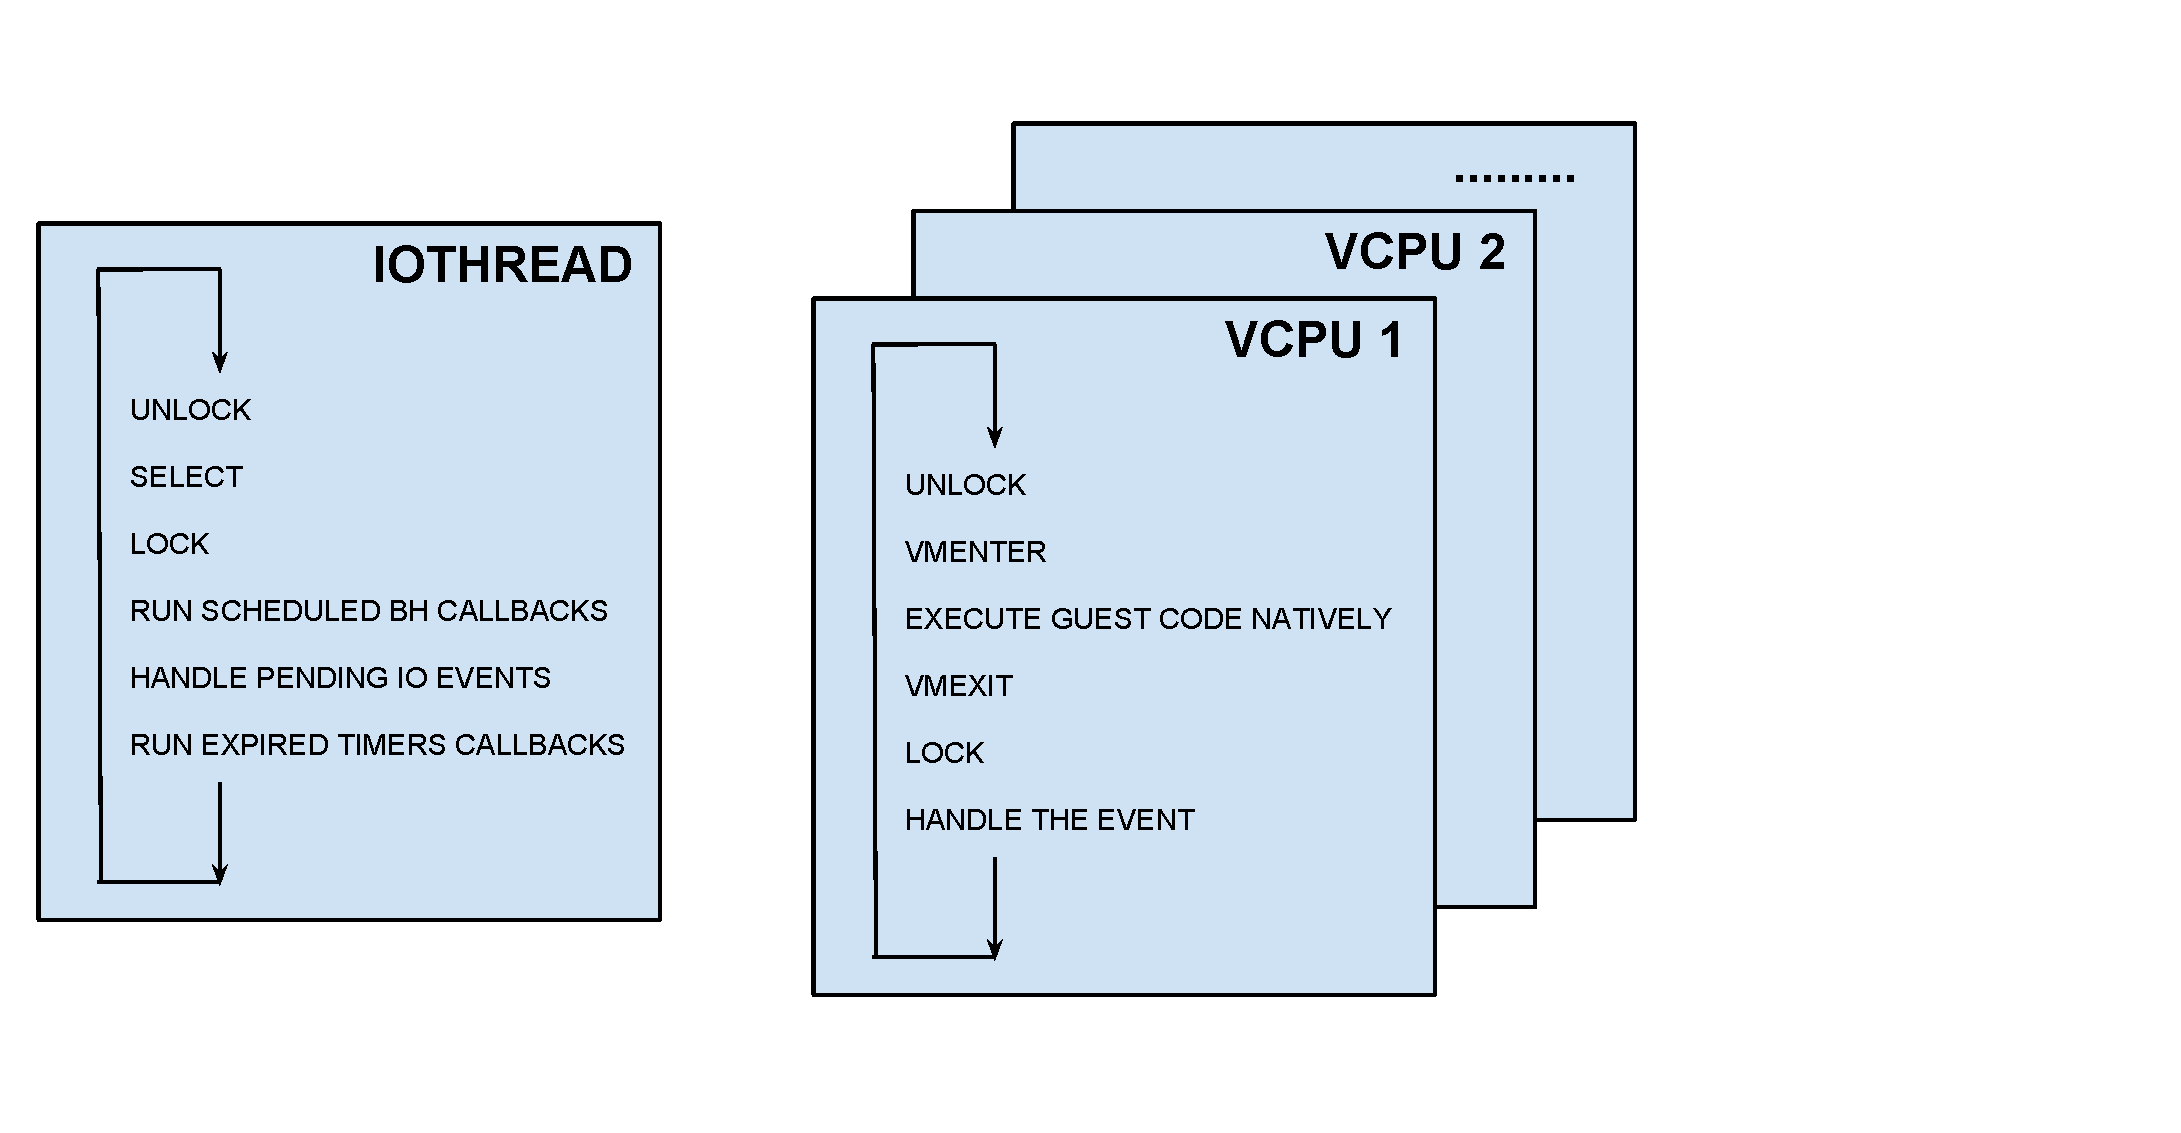
\includegraphics[width=1.0\columnwidth]{qemu-threads.pdf}
      \end{figure}
    \end{column}
  
    \begin{column}{0.5\textwidth}
    \begin{block}{QEMU is an event-loop}
      \begin{itemize}
	\pause
	\item A dedicated \emph{IOThread} executes the event-loop
	\pause
	\item A thread for each guest VCPU
      \end{itemize}
    \end{block}
    \end{column}
  \end{columns}
\end{frame}
  
\begin{frame}
\frametitle{QEMU-KVM internal structure}
    \begin{block}{KVM mechanics}
      \begin{itemize}
	\item VCPU access I/O or is interrupted $\rightarrow$ A world switch occurs
	\pause
	\item I/O emulation can be done both by VCPUs and by IOThread
	\pause
	\item Mutual exclusion required $\longrightarrow$ A \emph{Big-Lock} is employed
      \end{itemize}
    \end{block}
\end{frame}

\begin{frame}
\frametitle{QEMU networking}
  \begin{block}{Need for networking support}
      \begin{itemize}
	\item Guest OS thinks to deal with a physical network adapter $\rightarrow$ Uses the original driver
	\pause
	\item The network adapter is emulated by a QEMU \emph{network frontend}
	\pause
	\item A QEMU \emph{network backend} provides connectivity to the outside world
	\pause
	\item Frontend and backend exchange network packets
      \end{itemize}
    \end{block}
\end{frame}

\begin{frame}
\frametitle{QEMU networking}
    \begin{figure}
    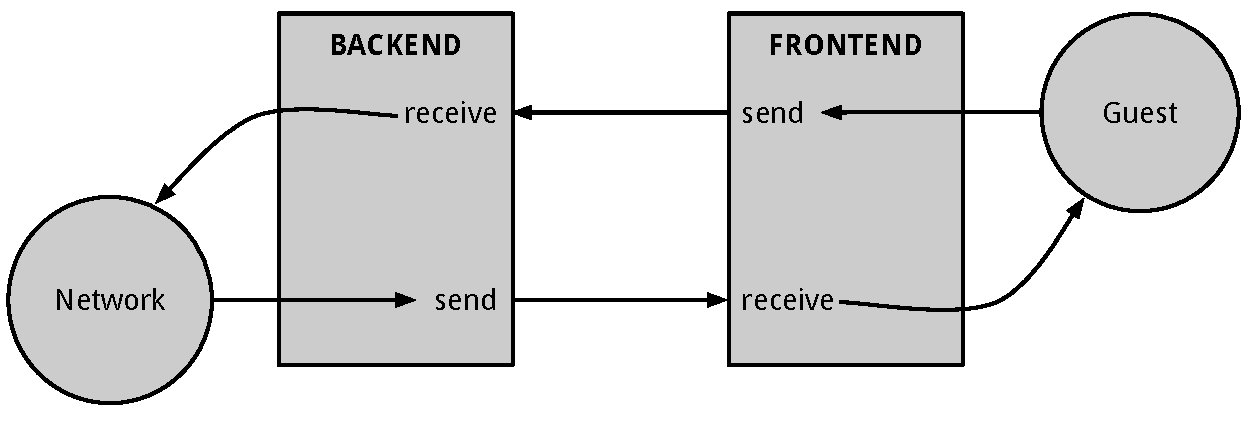
\includegraphics[width=.90\columnwidth]{frontend-backend.pdf}
    \end{figure}
\end{frame}

\begin{frame}
\frametitle{QEMU networking}

  \begin{columns}
    \begin{column}{0.5\textwidth}
      \begin{figure}
	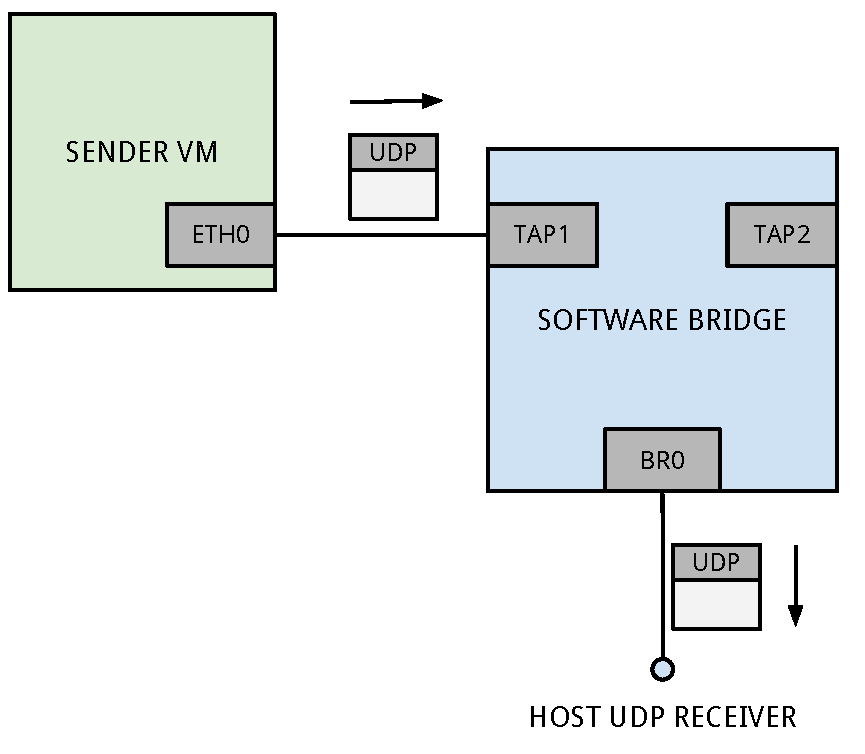
\includegraphics[width=1.0\columnwidth]{scenario-1.pdf}
      \end{figure}
    \end{column}
    \begin{column}{0.5\textwidth}
    \begin{block}{In this work}
      \begin{itemize}
	\item e1000 network adapter
	\pause
	\item The TAP backend (TAP devices)
	\pause
	\item Many TAP bridged together $\rightarrow$ Virtual LAN
      \end{itemize}
    \end{block}
    \end{column}
  \end{columns}
\end{frame}

\begin{frame}
\frametitle{The e1000 interface specification}
    \begin{figure}
      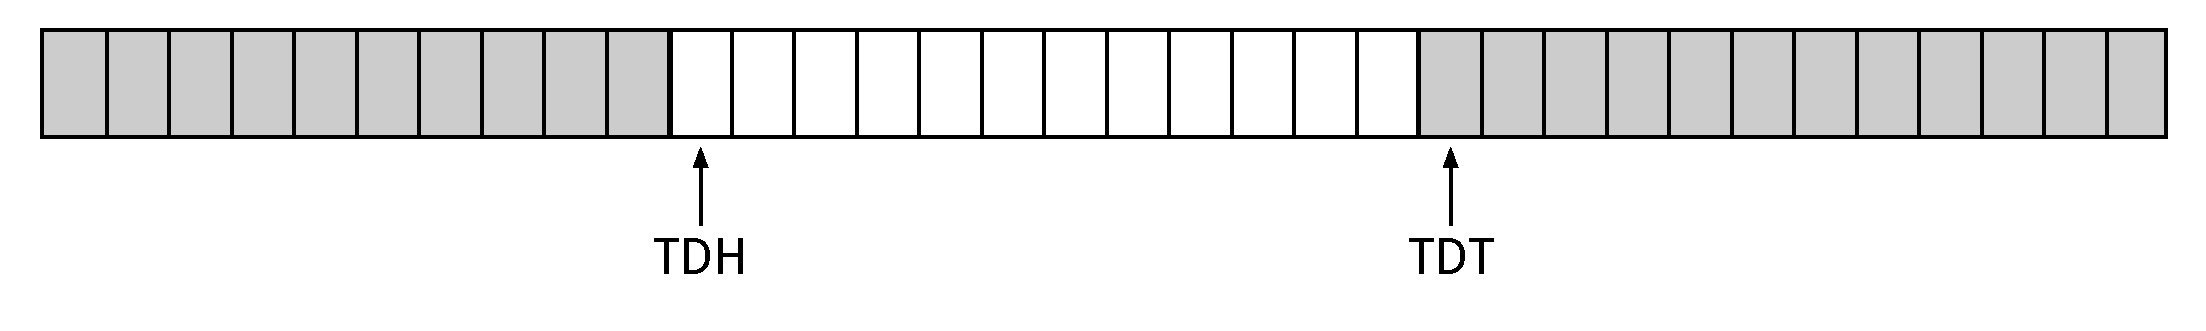
\includegraphics[width=1.0\columnwidth]{tx-ring.pdf}
    \end{figure}
    
    \begin{block}{How do driver and device exchange packets?}
      \begin{itemize}
	\item Two queue of descriptors (\emph{rings}): TX ring and RX ring
	\pause
	\item Each descriptor references a buffer
	\pause
	\item Driver inserts descriptors to give buffers to the device
	\pause
	\item Device uses the buffers and returns them to the driver
	\pause
	\item Synchronization is achieved using head/tail index registers
      \end{itemize}
    \end{block}
\end{frame}

%\begin{frame}
%\frametitle{QEMU e1000 emulation}
%  \begin{block}{How is emulation performed?}
%    \begin{enumerate}
%      \item A VCPU tries to access an e1000 register $\rightarrow$ The VPCU switches to host world
%      \pause
%      \item QEMU takes the control and invoke the e1000 frontend
%      \pause
%      \item The e1000 frontend emulates all the side effects of the register access
%    \end{enumerate}
%  \end{block}
%\end{frame}
   
\begin{frame}
\frametitle{TX/RX path}
  \begin{columns}
  \begin{column}{0.5\textwidth}
    \begin{figure}
      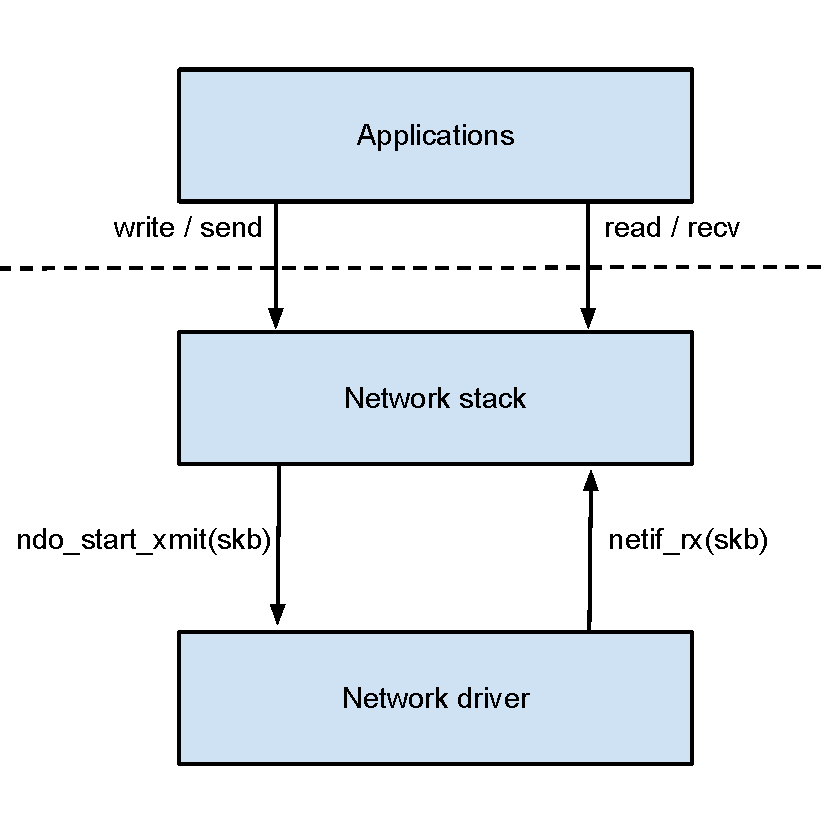
\includegraphics[width=1.0\columnwidth]{linux-interface.pdf}
    \end{figure}
  \end{column}

  \begin{column}{0.5\textwidth}
    \begin{block}{TX path}
      \begin{itemize}
	\item Packet to send $\rightarrow$ The kernel invokes the e1000 \texttt{ndo\_start\_xmit()} method
	\pause
	\item The driver inserts a new TX descriptor in the ring and updates the TDT register
      \end{itemize}
    \end{block}
  \end{column}
  \end{columns}
\end{frame}

\begin{frame}
\frametitle{TX/RX path}
  \begin{columns}
  \begin{column}{0.5\textwidth}
    \begin{figure}
      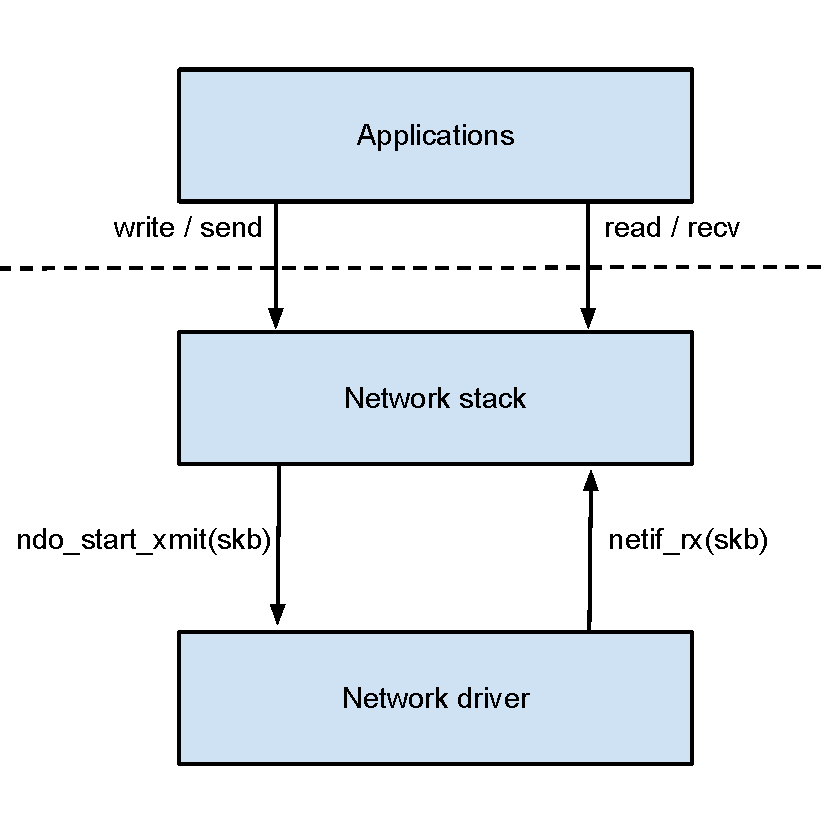
\includegraphics[width=1.0\columnwidth]{linux-interface.pdf}
    \end{figure}
  \end{column}
  
  \begin{column}{0.5\textwidth}
    \begin{block}{RX path}
      \begin{itemize}
	\item The adapter receives a packet into the RX ring $\rightarrow$ An interrupt is raised
	\pause
	\item The driver interrupt routine pushes the receive packet to the network stack
      \end{itemize}
    \end{block}
  \end{column}
  \end{columns}
\end{frame}


%=================================================================
\section{e1000 optimizations}
%=================================================================

\begin{frame}
\frametitle{Problems of the existing implementation}
    \begin{block}{TX statistics}
    \begin{center}
    \begin{tabular}{lrl}
      \textbf{Interrupt rate} & 20.6 & KHz\\
      \textbf{TX packet rate} & 20.6 & Kpps\\
      \textbf{TX notifications rate} & 20.6 & KHz\\
      \textbf{MMIO rate} & 123.4 & KHz\\
    \end{tabular}
    \end{center}
    \end{block}
    
    \begin{block}{RX statistics}
    \begin{center}
    \begin{tabular}{lrl}
      \textbf{Interrupt rate} & 14.3 & KHz\\
      \textbf{RX packet rate} & 14.4 & Kpps\\
      \textbf{RX notifications} & 14.3 & Mbps\\
      \textbf{MMIO rate} & 85.8 & KHz\\
    \end{tabular}
    \end{center}
    \end{block}
\end{frame}

\begin{frame}
\frametitle{Problems of the existing implementation}
    \begin{block}{What are the problems and bottlenecks?}
      \begin{itemize}
	\item Interrupt mitigation is not emulated
	\item 5 register accesses in the interrupt routine
	\item A TX notification for each TX packet
	\item A RX notification for each RX packet
	\item TX emulation is done synchronously
      \end{itemize}
    \end{block}
\end{frame}


\begin{frame}
\frametitle{Adding interrupt moderation}
    \begin{block}{Interrupt moderation patch}
      \begin{itemize}
	\item The e1000 frontend limits the Maximum Interrupt Rate $\rightarrow$ Interrupts are coalesced
	\pause
	\item To achieve that, we use a timer to delay the interrupts
	\pause
	\item The patch is only 50 lines of code
      \end{itemize}
    \end{block}
\end{frame}

\begin{frame}
\frametitle{Adding interrupt moderation}
    \begin{block}{TX statistics improvements}
      \begin{center}
      \begin{tabular}{lrcrl}
      \textbf{Interrupt rate} & 20.6 & $\rightarrow$ & 3.8 & KHz\\
      \textbf{TX packet rate} & 20.6 & $\rightarrow$ & 47.8 & Kpps\\
      \textbf{TX notifications rate} & 20.6 & $\rightarrow$ & 47.8 & KHz\\
      \textbf{MMIO rate} & 123.4 & $\rightarrow$ & 67.0 & KHz\\
      \end{tabular}
      \end{center}
    \end{block}
    
    \begin{block}{RX statistics improvements}
      \begin{center}
      \begin{tabular}{lrcrl}
	\textbf{Interrupt rate} & 14.3 & $\rightarrow$ & 3.8 & KHz\\
	\textbf{RX packet rate} & 14.4 & $\rightarrow$ & 137.1 & Kpps\\
	\textbf{RX notifications} & 14.3 & $\rightarrow$ & 10.3 & Mbps\\
	\textbf{MMIO rate} & 85.8 & $\rightarrow$ & 29.5 & KHz\\
      \end{tabular}
      \end{center}
    \end{block}
\end{frame}

\begin{frame}
\frametitle{Maximum TX packet rate vs MAIR}
  \begin{figure}
    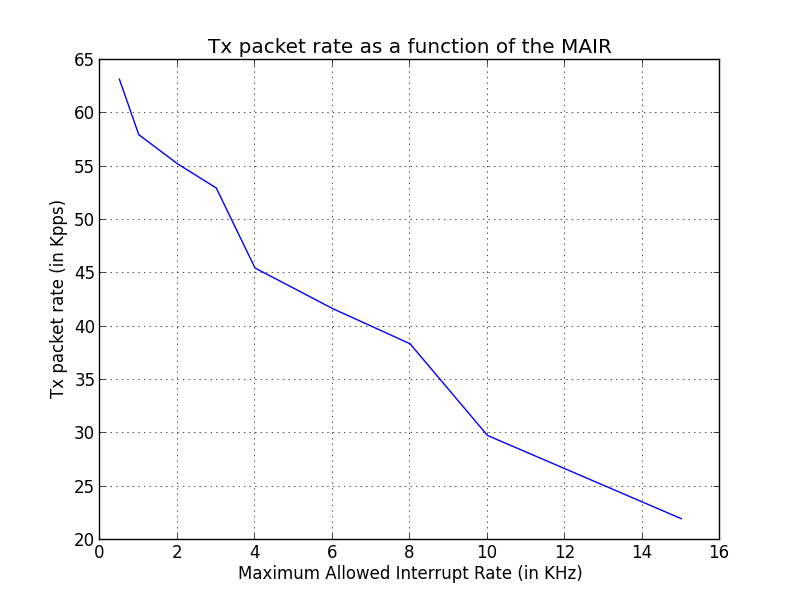
\includegraphics[width=0.75\columnwidth]{MAIR-vs-TXRate.png}
  \end{figure}
\end{frame}

\begin{frame}
\frametitle{Maximum RX packet rate vs MAIR}
  \begin{figure}
    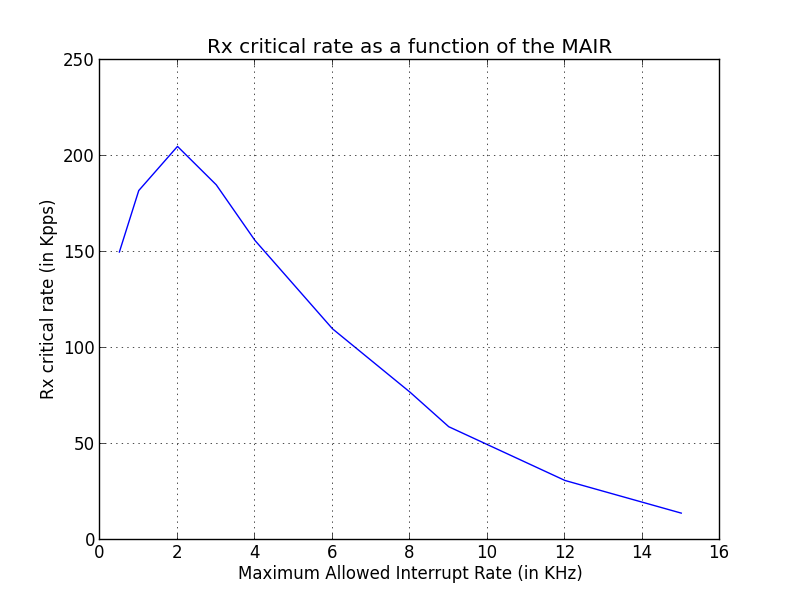
\includegraphics[width=0.75\columnwidth]{MAIR-vs-CR.png}
  \end{figure}
\end{frame}


\begin{frame}
\frametitle{Batching TX notifications}
    \begin{block}{TDT \emph{write batching} patch}
      \begin{itemize}
	\item The e1000 driver coalesces TX notifications
	\pause
	\item We don't notify if there is a pending TX interrupt
	\pause
	\item We use the e1000 interrupt routine to flush pending TX frames
	\pause
	\item The patch is only 35 lines of code
      \end{itemize}
    \end{block}
\end{frame}

\begin{frame}
\frametitle{Batching TX notifications}
    \begin{block}{TX statistics improvements w.r.t. moderation patch statistics}
      \begin{center}
      \begin{tabular}{lrcrl}
      \textbf{Interrupt rate} & 3.8 & $\rightarrow$ & 1.8 & KHz\\
      \textbf{TX packet rate} & 47.8 & $\rightarrow$ & 163.5 & Kpps\\
      \textbf{TX notifications rate} & 47.8 & $\rightarrow$ & 1.8 & KHz\\
      \textbf{MMIO rate} & 67.0 & $\rightarrow$ & 11.1 & KHz\\
      \end{tabular}
      \end{center}
    \end{block}
\end{frame}



%=================================================================
\section{A paravirtualized e1000}
%=================================================================

\begin{frame}
\frametitle{Full virtualization vs paravirtualization}
    \begin{block}{Full virtualization}
      \begin{itemize}
	\item The guest OS is unaware of being run in a Virtual Machine environment
	\pause
	\item Advantage: The hypervisor can support an unmodified OS
	\pause
	\item Disadvantage: Hypervisor implementation is complicated and inefficient
      \end{itemize}
    \end{block}
\end{frame}

\begin{frame}
\frametitle{Full virtualization vs paravirtualization}
    \begin{block}{Paravirtualization}
      \begin{itemize}
	\item The guest OS is aware of being under the control of an hypervisor
	\pause
	\item Guest and hypervisor can communicate in a simpler and more efficient way
	\pause
	\item MMIO accesses and interrupts are used \emph{only} for notifications
	\pause
	\item Data are exchanged only through shared memory
      \end{itemize}
    \end{block}
\end{frame}

\begin{frame}
\frametitle{The Virtio standard}
  \begin{columns}
    \begin{column}{0.5\textwidth}
      \begin{figure}
	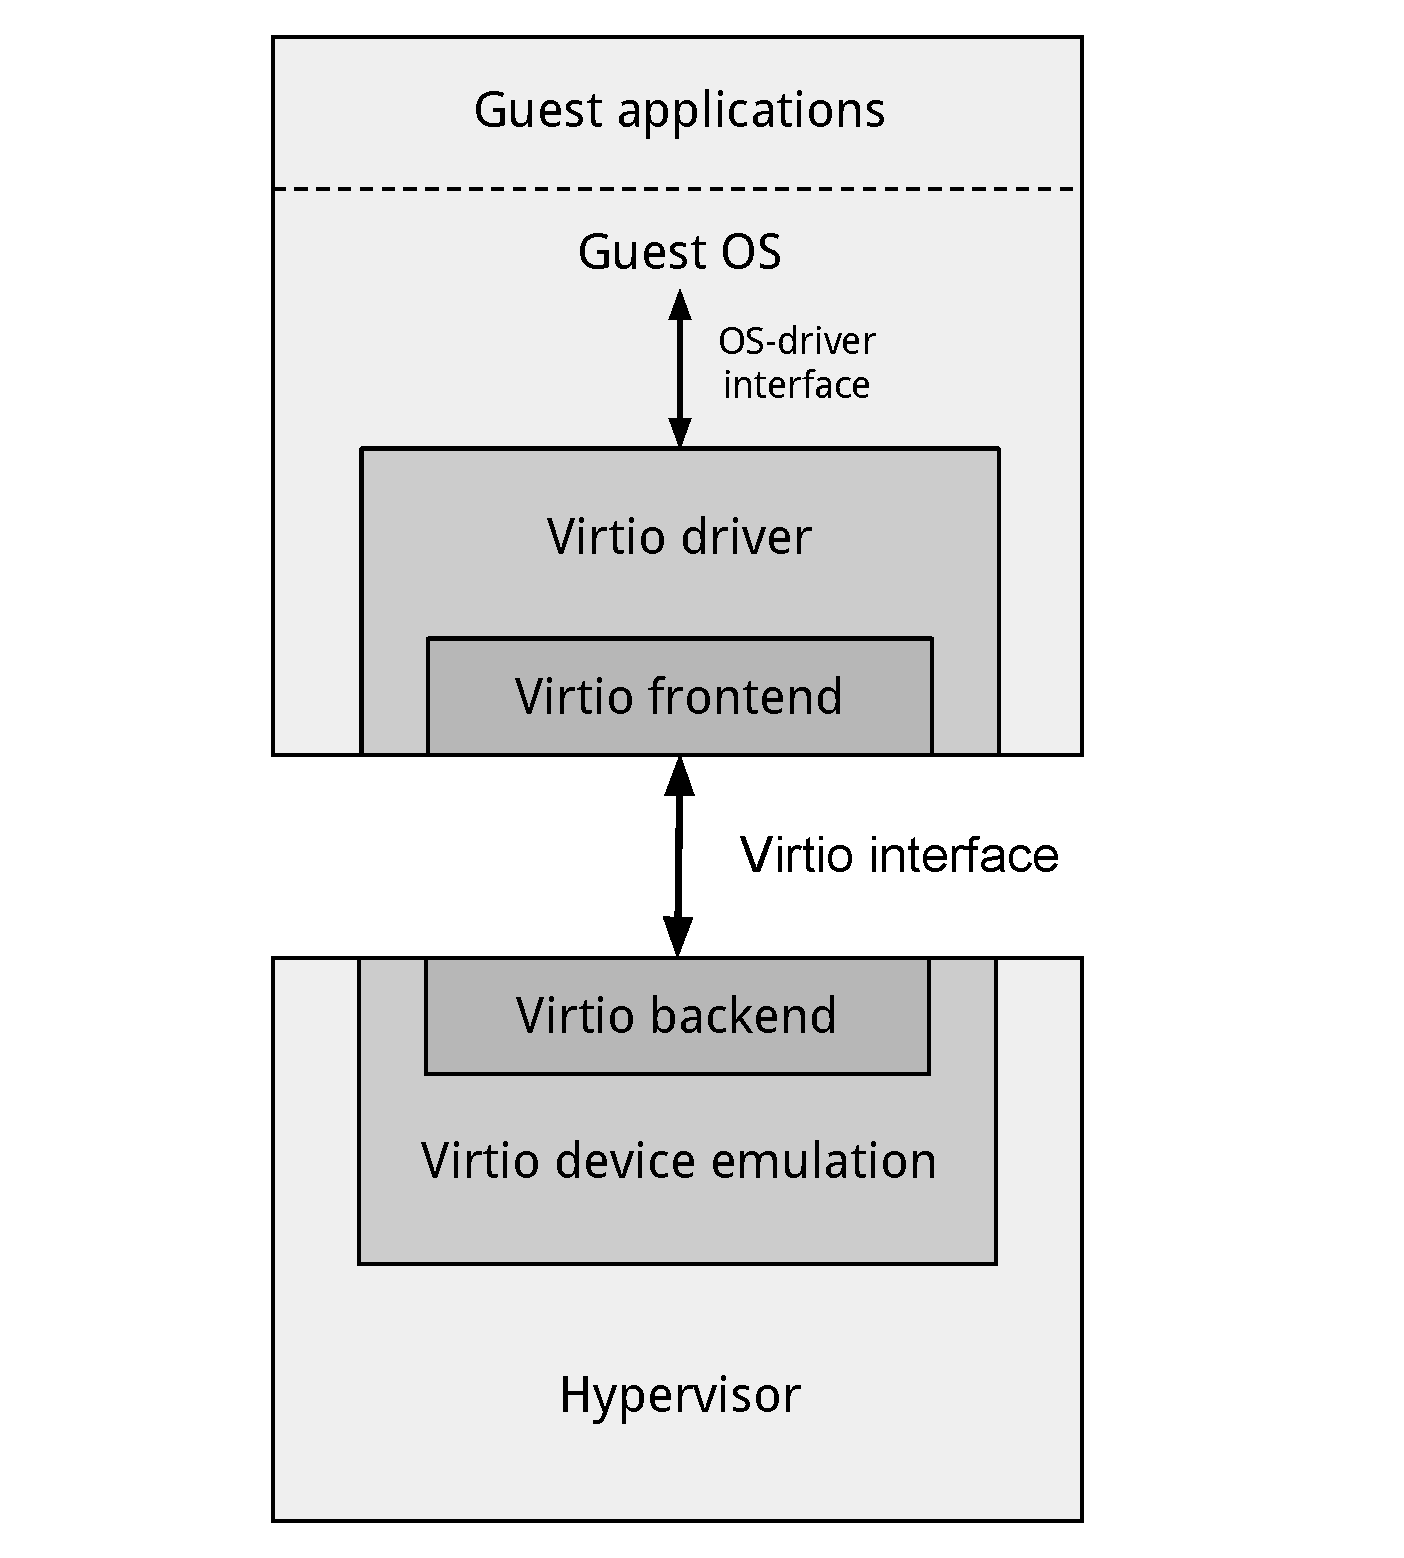
\includegraphics[width=1.0\columnwidth]{virtio.pdf}
      \end{figure}
    \end{column}
  
    \begin{column}{0.5\textwidth}
    \begin{block}{Virtio}
      \begin{itemize}
	\item A \emph{de facto} standard for I/O paravirtualization
	\pause
	\item A set of new efficient device drivers/emulators
	\pause
	\item Increase code reuse across devices and platforms
      \end{itemize}
    \end{block}
    \end{column}
  \end{columns}
\end{frame}

\begin{frame}
    \begin{figure}
      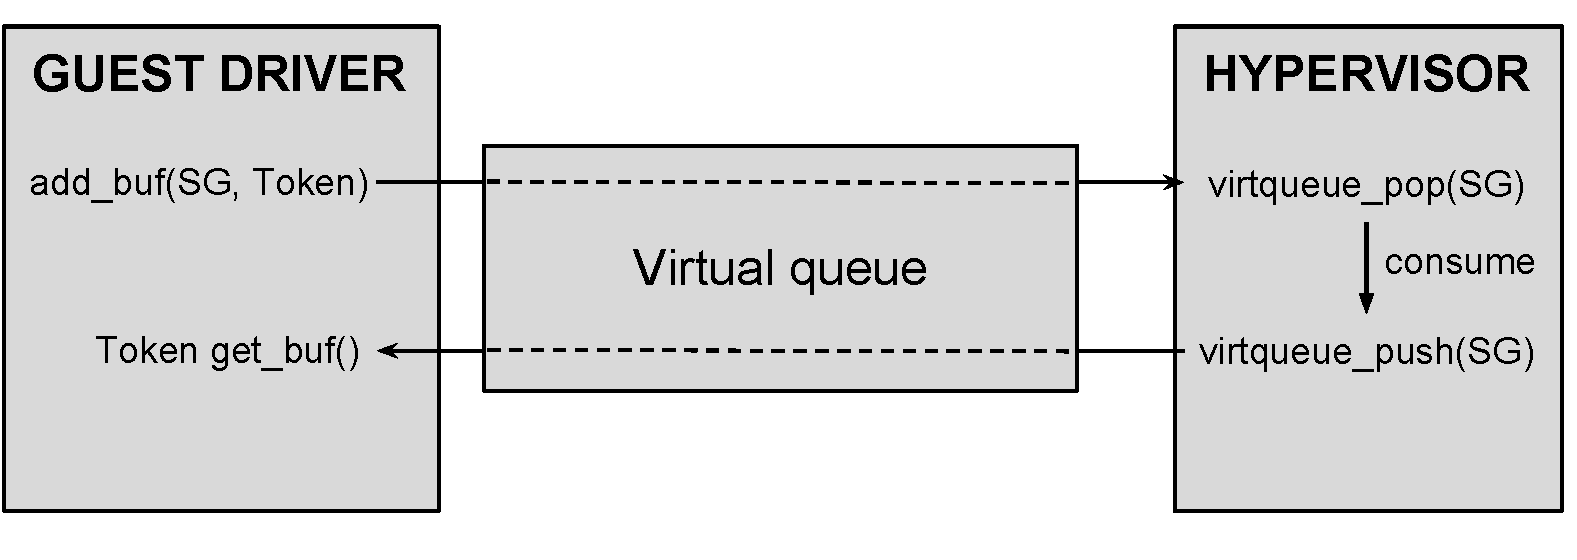
\includegraphics[width=.9\columnwidth]{virtqueue.pdf}
      \caption{Driver and hypervisor can exchange data through a virtual queue}
    \end{figure}
\end{frame}

\begin{frame}
\frametitle{Porting the paravirtualization concept to e1000}
    \begin{block}{Notification-efficient producer/consumer communication}
      \begin{itemize}
	\item e1000 index registers exported to a shared memory area (\emph{Communication Status Block})
	\pause
	\item Added flags to enable/disable TX/RX notifications
	\pause
	\item Two Producer/consumer couples (PCCs) for the TX path and two PCCs for the RX path
	\pause
	\item The producer notifies the consumer only when the consumer is not active
	\pause
	\item Consumer work is done asynchronously w.r.t. the producer and with notifications disabled
	\pause
	\item If the consumer is faster notification moderation is required
      \end{itemize}
    \end{block}
\end{frame}
  
\begin{frame}
    \begin{block}{Paravirtualization patch}
      \begin{itemize}
	\item Both e1000 driver and e1000 emulation must be patched
	\item About 100 lines of code in the hypervisor
	\item About 40 lines in the Linux kernel
      \end{itemize}
    \end{block}
\end{frame}

\begin{frame}
    \begin{block}{TX statistics improvements w.r.t. moderation patch statistics}
      \begin{center}
      \begin{tabular}{lrcrl}
      \textbf{Interrupt rate} & 3.8 & $\rightarrow$ & 0.37 & KHz\\
      \textbf{TX packet rate} & 47.8 & $\rightarrow$ & 183.4 & Kpps\\
      \textbf{TX notifications rate} & 47.8 & $\rightarrow$ & 0.4 & KHz\\
      \textbf{MMIO rate} & 67.0 & $\rightarrow$ & 1.53 & KHz\\
      \end{tabular}
      \end{center}
    \end{block}
    
    \begin{block}{RX statistics improvements w.r.t. moderation patch statistics}
      \begin{center}
      \begin{tabular}{lrcrl}
	\textbf{Interrupt rate} & 3.8 & $\rightarrow$ & 3.8 & KHz\\
	\textbf{RX packet rate} & 137.1 & $\rightarrow$ & 317.3 & Kpps\\
	\textbf{RX notifications} & 10.3 & $\rightarrow$ & 0.002 & Mbps\\
 	\textbf{MMIO rate} & 29.5 & $\rightarrow$ & 11.1 & KHz\\
      \end{tabular}
      \end{center}
    \end{block}
\end{frame}


%=================================================================
\section{Conclusions and future work}
%=================================================================
\begin{frame}
  \frametitle{Summary}
    \begin{block}{}
      \begin{center}
      \begin{tabular}{lrcrl}
	\textbf{Combination} 			& \textbf{TX} 	& \textbf{RX} 	& \\
	e1000 					&	20.6	&  	14.4	& KHz\\
	e1000 + moderation 			& 	47.8 	& 	137.1 	& KHz\\
	e1000 + moderation + batching 		&  	163.5	& 	137.1 	& KHz\\
	e1000 + moderation + paravirtualization	&	183.4	&	317.3	& KHz\\
 	Virtio 					& 	158.1	& 	103.0	& KHz\\
      \end{tabular}
      \end{center}
    \end{block}
\end{frame}

\begin{frame}
\frametitle{Conclusions}
  \begin{block}{}
    \begin{itemize}
      \item Some simple modifications to the e1000 framework lead to big performance improvements
      \pause
      \item TX path: $8.9\times$ speed-up
      \item RX path: $22\times$ speed-up
    \end{itemize}
  \end{block}
\end{frame}

\begin{frame}
\frametitle{Future work}
  \begin{block}{More can be done to optimize e1000 performance in VM systems}
    \begin{itemize}
      \item Remove redundant packet copies in the TX path
      \pause
      \item Euristics to improve latency, bypassing interrupt moderation
      \pause
      \item Explore TSO/GSO to improve TCP throughput
    \end{itemize}
  \end{block}
\end{frame}


\begin{frame}
\begin{center}
{\Large The end}
\end{center}

\end{frame}
\end{document}
